% !TeX root = relatorio.tex
\documentclass[12pt,a4paper]{article}

\usepackage[T1]{fontenc}
\usepackage[utf8]{inputenc}
\usepackage[brazilian]{babel}
\usepackage{lmodern}
\usepackage[a4paper,margin=2.5cm]{geometry}
\usepackage{amsmath}
\usepackage{amssymb}
\usepackage{graphicx}
\usepackage{float}
\usepackage{booktabs}
\usepackage{hyperref}
\usepackage{xcolor}
\usepackage{subcaption}

\hypersetup{
  colorlinks=true,
  linkcolor=blue,
  urlcolor=blue,
  pdftitle={Relatorio do Trabalho 3},
  pdfauthor={Gustavo Shoiti Sonoda}
}
\urlstyle{tt}

\renewcommand{\contentsname}{Sumário}
\setlength{\parindent}{0pt}
\setlength{\parskip}{0.7em}
\linespread{1.05}

\newcommand{\arquivo}[1]{\nolinkurl{#1}}
\newcommand{\campo}[2]{\textbf{#1.} #2\par}
\newcommand{\figdir}[1]{figuras/#1}
\newcommand{\figanalise}[1]{figuras/analise_#1}

\begin{document}
\hypersetup{pageanchor=false}
\pagenumbering{gobble}

\begin{titlepage}
  \centering

  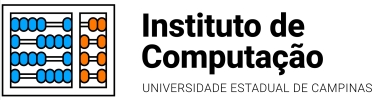
\includegraphics[width=0.24\textwidth]{figuras/logo_ic.png}\par
  \vspace{0.8cm}
  {\large Universidade Estadual de Campinas\par}
  {\large Instituto de Computação\par}

  \vspace{1.5cm}

  {\Large \textbf{Relatório de Implementação do Trabalho 3}\par}
  \vspace{0.5cm}
  {\large Introdução ao Processamento Digital de Imagens (MC920/MO443)\par}
  \vspace{1.2cm}

  {\large Relatório de implementação desenvolvido para a disciplina\\
    Introdução ao Processamento Digital de Imagens.\par}

  \vspace{1.5cm}

  \begin{flushleft}
    \textbf{Professor:} Hélio Pedrini\\
    \textbf{Aluno:} Gustavo Shoiti Sonoda\\
    \textbf{RA:} 217579\\
  \end{flushleft}

  \vfill

  Campinas -- São Paulo\\
  \today
\end{titlepage}

\tableofcontents
\newpage
\hypersetup{pageanchor=true}
\pagenumbering{arabic}

% ---------------------------------------------------------------------------
\section{Introdução}
\label{sec:introducao}
% ---------------------------------------------------------------------------

O Trabalho~3 da disciplina MC920/MO443 propõe a exploração da transformada de
Fourier bidimensional (2D-FFT) como ferramenta de análise estrutural de imagens.
A transformada de Fourier permite representar uma imagem no domínio da frequência,
revelando padrões relacionados a escala, direção e periodicidade que não são
diretamente observáveis no domínio espacial.

O trabalho está dividido em duas partes principais:

\begin{itemize}
  \item \textbf{Análise~1} (Seção~\ref{sec:espectro}): cálculo do espectro de
        magnitude da FFT 2D em escala logarítmica, construção do histograma
        angular de energia e identificação das orientações dominantes.
  \item \textbf{Análise~2} (Seção~\ref{sec:invariancia}): verificação experimental
        das propriedades de invariância da transformada de Fourier frente a
        translações, rotações e mudanças de escala.
\end{itemize}

As imagens de entrada são os arquivos PGM disponibilizados no servidor da Unicamp
(\url{http://www.ic.unicamp.br/~helio/imagens_pgm/}), e todas as saídas são
geradas no formato PNG.

% ---------------------------------------------------------------------------
\section{Materiais e Métodos}
\label{sec:materiais}
% ---------------------------------------------------------------------------

\subsection{Ambiente e organização}

\campo{Linguagem e bibliotecas}{A implementação foi desenvolvida em Python~3.
O projeto utiliza \textit{Pillow} para leitura de imagens PGM e gravação de PNG,
\textit{NumPy} para as operações com arrays e a FFT (\texttt{numpy.fft}),
\textit{SciPy} (\texttt{scipy.ndimage}) para as transformações geométricas e
\textit{Matplotlib} para geração dos gráficos e visualizações do espectro.}

\campo{Organização do código}{Cada análise está encapsulada em um módulo
independente dentro de \arquivo{src/trabalho\_03/}:
\arquivo{analise\_01\_espectro\_histograma/main.py} e
\arquivo{analise\_02\_invariancia/main.py}.
A infraestrutura compartilhada (gerenciamento de caminhos, download de entradas,
benchmarks e relatório) reside em \arquivo{src/common/}.}

\campo{Imagens de entrada}{As sete imagens PGM utilizadas são:
\textit{baboon}, \textit{fiducial}, \textit{monarch}, \textit{peppers},
\textit{retina}, \textit{sonnet} e \textit{wedge}.
Todas são monocromáticas (8~bits por pixel).}

\subsection{Representação das imagens}

No módulo de análise, as imagens são carregadas como \texttt{list[list[int]]}
(lista de listas de inteiros no intervalo $[0, 255]$) pela função
\texttt{load\_grayscale\_image} de \arquivo{src/common/image\_io.py}.
Antes de aplicar a FFT, o array é convertido para \texttt{numpy.ndarray} de
tipo \texttt{float64}.

\subsection{Transformada de Fourier 2D}

A FFT 2D de uma imagem $f(x, y)$ de dimensões $M \times N$ é dada por:

\begin{equation}
  F(u, v) = \sum_{x=0}^{M-1} \sum_{y=0}^{N-1}
            f(x, y)\, e^{-j2\pi\left(\frac{ux}{M} + \frac{vy}{N}\right)}
\end{equation}

O espectro de magnitude centrado é calculado como $|F_{\text{shift}}(u,v)|$,
onde $F_{\text{shift}}$ desloca a componente DC para o centro da imagem
(\texttt{numpy.fft.fftshift}).
A escala logarítmica $\log(1 + |F|)$ é aplicada para comprimir o intervalo
dinâmico e tornar visíveis as frequências de baixa energia.

\subsection{Histograma angular de energia}

Para cada ponto $(u, v)$ do espectro centrado, calcula-se o ângulo relativo ao
centro $(u_c, v_c)$:

\begin{equation}
  \theta(u, v) = \operatorname{atan2}(v - v_c,\; u - u_c) \in [-\pi, \pi]
\end{equation}

O ângulo é mapeado para um dos $N_{\text{bins}}$ intervalos angulares, e a
magnitude espectral correspondente é acumulada nesse bin.
O resultado é um histograma que descreve como a energia está distribuída pelas
diferentes direções da imagem.

% ---------------------------------------------------------------------------
\section{Análise 1: Espectro de Magnitude e Histograma Angular}
\label{sec:espectro}
% ---------------------------------------------------------------------------

\subsection{Descrição}

% TODO: descreva aqui sua implementação de compute_fft_magnitude_spectrum,
%       compute_log_spectrum, compute_angular_histogram e
%       identify_dominant_orientations. Explique as escolhas de parâmetros
%       (número de bins, raio mínimo descartado, etc.) e discuta os resultados.

\subsection{Resultados — baboon}

\begin{figure}[H]
  \centering
  \begin{subfigure}[b]{0.45\textwidth}
    \centering
    \includegraphics[width=\textwidth]{\figanalise{01_espectro_histograma}/fourier_baboon_original.png}
    \caption{Imagem original}
  \end{subfigure}
  \hfill
  \begin{subfigure}[b]{0.45\textwidth}
    \centering
    \includegraphics[width=\textwidth]{\figanalise{01_espectro_histograma}/fourier_baboon_espectro_log.png}
    \caption{Espectro (log)}
  \end{subfigure}
  \caption{Baboon — imagem original e espectro de magnitude logarítmico.}
\end{figure}

\begin{figure}[H]
  \centering
  \includegraphics[width=0.65\textwidth]{\figanalise{01_espectro_histograma}/fourier_baboon_histograma_angular.png}
  \caption{Baboon — histograma angular de energia.}
\end{figure}

\begin{figure}[H]
  \centering
  \includegraphics[width=0.5\textwidth]{\figanalise{01_espectro_histograma}/fourier_baboon_orientacoes_dominantes.png}
  \caption{Baboon — orientações dominantes sobrepostas ao espectro.}
\end{figure}

% TODO: repita o padrão acima para as demais imagens (fiducial, monarch,
%       peppers, retina, sonnet, wedge) e adicione discussão comparativa.

\subsection{Resultados — fiducial}

\begin{figure}[H]
  \centering
  \begin{subfigure}[b]{0.45\textwidth}
    \centering
    \includegraphics[width=\textwidth]{\figanalise{01_espectro_histograma}/fourier_fiducial_original.png}
    \caption{Imagem original}
  \end{subfigure}
  \hfill
  \begin{subfigure}[b]{0.45\textwidth}
    \centering
    \includegraphics[width=\textwidth]{\figanalise{01_espectro_histograma}/fourier_fiducial_espectro_log.png}
    \caption{Espectro (log)}
  \end{subfigure}
  \caption{Fiducial — imagem original e espectro de magnitude logarítmico.}
\end{figure}

\begin{figure}[H]
  \centering
  \includegraphics[width=0.65\textwidth]{\figanalise{01_espectro_histograma}/fourier_fiducial_histograma_angular.png}
  \caption{Fiducial — histograma angular de energia.}
\end{figure}

\begin{figure}[H]
  \centering
  \includegraphics[width=0.5\textwidth]{\figanalise{01_espectro_histograma}/fourier_fiducial_orientacoes_dominantes.png}
  \caption{Fiducial — orientações dominantes sobrepostas ao espectro.}
\end{figure}

\subsection{Resultados — monarch}

\begin{figure}[H]
  \centering
  \begin{subfigure}[b]{0.45\textwidth}
    \centering
    \includegraphics[width=\textwidth]{\figanalise{01_espectro_histograma}/fourier_monarch_original.png}
    \caption{Imagem original}
  \end{subfigure}
  \hfill
  \begin{subfigure}[b]{0.45\textwidth}
    \centering
    \includegraphics[width=\textwidth]{\figanalise{01_espectro_histograma}/fourier_monarch_espectro_log.png}
    \caption{Espectro (log)}
  \end{subfigure}
  \caption{Monarch — imagem original e espectro de magnitude logarítmico.}
\end{figure}

\begin{figure}[H]
  \centering
  \includegraphics[width=0.65\textwidth]{\figanalise{01_espectro_histograma}/fourier_monarch_histograma_angular.png}
  \caption{Monarch — histograma angular de energia.}
\end{figure}

\begin{figure}[H]
  \centering
  \includegraphics[width=0.5\textwidth]{\figanalise{01_espectro_histograma}/fourier_monarch_orientacoes_dominantes.png}
  \caption{Monarch — orientações dominantes sobrepostas ao espectro.}
\end{figure}

\subsection{Resultados — peppers}

\begin{figure}[H]
  \centering
  \begin{subfigure}[b]{0.45\textwidth}
    \centering
    \includegraphics[width=\textwidth]{\figanalise{01_espectro_histograma}/fourier_peppers_original.png}
    \caption{Imagem original}
  \end{subfigure}
  \hfill
  \begin{subfigure}[b]{0.45\textwidth}
    \centering
    \includegraphics[width=\textwidth]{\figanalise{01_espectro_histograma}/fourier_peppers_espectro_log.png}
    \caption{Espectro (log)}
  \end{subfigure}
  \caption{Peppers — imagem original e espectro de magnitude logarítmico.}
\end{figure}

\begin{figure}[H]
  \centering
  \includegraphics[width=0.65\textwidth]{\figanalise{01_espectro_histograma}/fourier_peppers_histograma_angular.png}
  \caption{Peppers — histograma angular de energia.}
\end{figure}

\begin{figure}[H]
  \centering
  \includegraphics[width=0.5\textwidth]{\figanalise{01_espectro_histograma}/fourier_peppers_orientacoes_dominantes.png}
  \caption{Peppers — orientações dominantes sobrepostas ao espectro.}
\end{figure}

\subsection{Resultados — retina}

\begin{figure}[H]
  \centering
  \begin{subfigure}[b]{0.45\textwidth}
    \centering
    \includegraphics[width=\textwidth]{\figanalise{01_espectro_histograma}/fourier_retina_original.png}
    \caption{Imagem original}
  \end{subfigure}
  \hfill
  \begin{subfigure}[b]{0.45\textwidth}
    \centering
    \includegraphics[width=\textwidth]{\figanalise{01_espectro_histograma}/fourier_retina_espectro_log.png}
    \caption{Espectro (log)}
  \end{subfigure}
  \caption{Retina — imagem original e espectro de magnitude logarítmico.}
\end{figure}

\begin{figure}[H]
  \centering
  \includegraphics[width=0.65\textwidth]{\figanalise{01_espectro_histograma}/fourier_retina_histograma_angular.png}
  \caption{Retina — histograma angular de energia.}
\end{figure}

\begin{figure}[H]
  \centering
  \includegraphics[width=0.5\textwidth]{\figanalise{01_espectro_histograma}/fourier_retina_orientacoes_dominantes.png}
  \caption{Retina — orientações dominantes sobrepostas ao espectro.}
\end{figure}

\subsection{Resultados — sonnet}

\begin{figure}[H]
  \centering
  \begin{subfigure}[b]{0.45\textwidth}
    \centering
    \includegraphics[width=\textwidth]{\figanalise{01_espectro_histograma}/fourier_sonnet_original.png}
    \caption{Imagem original}
  \end{subfigure}
  \hfill
  \begin{subfigure}[b]{0.45\textwidth}
    \centering
    \includegraphics[width=\textwidth]{\figanalise{01_espectro_histograma}/fourier_sonnet_espectro_log.png}
    \caption{Espectro (log)}
  \end{subfigure}
  \caption{Sonnet — imagem original e espectro de magnitude logarítmico.}
\end{figure}

\begin{figure}[H]
  \centering
  \includegraphics[width=0.65\textwidth]{\figanalise{01_espectro_histograma}/fourier_sonnet_histograma_angular.png}
  \caption{Sonnet — histograma angular de energia.}
\end{figure}

\begin{figure}[H]
  \centering
  \includegraphics[width=0.5\textwidth]{\figanalise{01_espectro_histograma}/fourier_sonnet_orientacoes_dominantes.png}
  \caption{Sonnet — orientações dominantes sobrepostas ao espectro.}
\end{figure}

\subsection{Resultados — wedge}

\begin{figure}[H]
  \centering
  \begin{subfigure}[b]{0.45\textwidth}
    \centering
    \includegraphics[width=\textwidth]{\figanalise{01_espectro_histograma}/fourier_wedge_original.png}
    \caption{Imagem original}
  \end{subfigure}
  \hfill
  \begin{subfigure}[b]{0.45\textwidth}
    \centering
    \includegraphics[width=\textwidth]{\figanalise{01_espectro_histograma}/fourier_wedge_espectro_log.png}
    \caption{Espectro (log)}
  \end{subfigure}
  \caption{Wedge — imagem original e espectro de magnitude logarítmico.}
\end{figure}

\begin{figure}[H]
  \centering
  \includegraphics[width=0.65\textwidth]{\figanalise{01_espectro_histograma}/fourier_wedge_histograma_angular.png}
  \caption{Wedge — histograma angular de energia.}
\end{figure}

\begin{figure}[H]
  \centering
  \includegraphics[width=0.5\textwidth]{\figanalise{01_espectro_histograma}/fourier_wedge_orientacoes_dominantes.png}
  \caption{Wedge — orientações dominantes sobrepostas ao espectro.}
\end{figure}

\subsection{Discussão}

% TODO: discuta as orientações dominantes encontradas em cada imagem.
%       Explique como a estrutura visual da imagem se reflete no espectro
%       e no histograma angular. Compare imagens com padrões regulares
%       (ex.: wedge, fiducial) com imagens naturais (ex.: baboon, monarch).

% ---------------------------------------------------------------------------
\section{Análise 2: Invariância da FFT sob Transformações Geométricas}
\label{sec:invariancia}
% ---------------------------------------------------------------------------

\subsection{Descrição}

% TODO: descreva sua implementação de translate_image, rotate_image e
%       scale_image. Indique os parâmetros utilizados (deslocamento em pixels,
%       ângulo, fator de escala) e explique o comportamento esperado de cada
%       transformação no domínio da frequência.

\subsection{Propriedades teóricas esperadas}

\begin{itemize}
  \item \textbf{Translação:} o espectro de magnitude $|F(u,v)|$ é invariante à
        translação espacial. Apenas a fase é alterada. Isso ocorre porque a
        translação corresponde a uma multiplicação por um fator de fase no
        domínio da frequência.

  \item \textbf{Rotação:} uma rotação de $\theta$ graus na imagem espacial
        causa uma rotação de $\theta$ graus no espectro de magnitude. O padrão
        de energia angular é preservado, mas girado.

  \item \textbf{Mudança de escala:} comprimir a imagem (fator $<1$) espalha
        as frequências radialmente (a imagem menor tem componentes de frequência
        mais altas no espectro). Expandir a imagem (fator $>1$) concentra as
        frequências próximas ao centro.
\end{itemize}

\subsection{Resultados — baboon}

\begin{figure}[H]
  \centering
  \begin{subfigure}[b]{0.45\textwidth}
    \centering
    \includegraphics[width=\textwidth]{\figanalise{02_invariancia}/inv_baboon_original.png}
    \caption{Original}
  \end{subfigure}
  \hfill
  \begin{subfigure}[b]{0.45\textwidth}
    \centering
    \includegraphics[width=\textwidth]{\figanalise{02_invariancia}/inv_baboon_espectro_original.png}
    \caption{Espectro original}
  \end{subfigure}

  \begin{subfigure}[b]{0.45\textwidth}
    \centering
    \includegraphics[width=\textwidth]{\figanalise{02_invariancia}/inv_baboon_translacao.png}
    \caption{Após translação}
  \end{subfigure}
  \hfill
  \begin{subfigure}[b]{0.45\textwidth}
    \centering
    \includegraphics[width=\textwidth]{\figanalise{02_invariancia}/inv_baboon_espectro_translacao.png}
    \caption{Espectro após translação}
  \end{subfigure}

  \begin{subfigure}[b]{0.45\textwidth}
    \centering
    \includegraphics[width=\textwidth]{\figanalise{02_invariancia}/inv_baboon_rotacao.png}
    \caption{Após rotação}
  \end{subfigure}
  \hfill
  \begin{subfigure}[b]{0.45\textwidth}
    \centering
    \includegraphics[width=\textwidth]{\figanalise{02_invariancia}/inv_baboon_espectro_rotacao.png}
    \caption{Espectro após rotação}
  \end{subfigure}

  \begin{subfigure}[b]{0.45\textwidth}
    \centering
    \includegraphics[width=\textwidth]{\figanalise{02_invariancia}/inv_baboon_escala.png}
    \caption{Após mudança de escala}
  \end{subfigure}
  \hfill
  \begin{subfigure}[b]{0.45\textwidth}
    \centering
    \includegraphics[width=\textwidth]{\figanalise{02_invariancia}/inv_baboon_espectro_escala.png}
    \caption{Espectro após mudança de escala}
  \end{subfigure}

  \caption{Baboon — invariância da FFT sob transformações geométricas.}
\end{figure}

% TODO: repita o padrão acima para as demais imagens (fiducial, monarch,
%       peppers, retina, sonnet, wedge).

\subsection{Resultados — fiducial}

\begin{figure}[H]
  \centering
  \begin{subfigure}[b]{0.45\textwidth}
    \centering
    \includegraphics[width=\textwidth]{\figanalise{02_invariancia}/inv_fiducial_original.png}
    \caption{Original}
  \end{subfigure}
  \hfill
  \begin{subfigure}[b]{0.45\textwidth}
    \centering
    \includegraphics[width=\textwidth]{\figanalise{02_invariancia}/inv_fiducial_espectro_original.png}
    \caption{Espectro original}
  \end{subfigure}

  \begin{subfigure}[b]{0.45\textwidth}
    \centering
    \includegraphics[width=\textwidth]{\figanalise{02_invariancia}/inv_fiducial_translacao.png}
    \caption{Após translação}
  \end{subfigure}
  \hfill
  \begin{subfigure}[b]{0.45\textwidth}
    \centering
    \includegraphics[width=\textwidth]{\figanalise{02_invariancia}/inv_fiducial_espectro_translacao.png}
    \caption{Espectro após translação}
  \end{subfigure}

  \begin{subfigure}[b]{0.45\textwidth}
    \centering
    \includegraphics[width=\textwidth]{\figanalise{02_invariancia}/inv_fiducial_rotacao.png}
    \caption{Após rotação}
  \end{subfigure}
  \hfill
  \begin{subfigure}[b]{0.45\textwidth}
    \centering
    \includegraphics[width=\textwidth]{\figanalise{02_invariancia}/inv_fiducial_espectro_rotacao.png}
    \caption{Espectro após rotação}
  \end{subfigure}

  \begin{subfigure}[b]{0.45\textwidth}
    \centering
    \includegraphics[width=\textwidth]{\figanalise{02_invariancia}/inv_fiducial_escala.png}
    \caption{Após mudança de escala}
  \end{subfigure}
  \hfill
  \begin{subfigure}[b]{0.45\textwidth}
    \centering
    \includegraphics[width=\textwidth]{\figanalise{02_invariancia}/inv_fiducial_espectro_escala.png}
    \caption{Espectro após mudança de escala}
  \end{subfigure}

  \caption{Fiducial — invariância da FFT sob transformações geométricas.}
\end{figure}

% TODO: adicionar monarch, peppers, retina, sonnet, wedge seguindo o mesmo padrão.

\subsection{Discussão}

% TODO: discuta se as propriedades teóricas foram verificadas
%       experimentalmente. Identifique e explique quaisquer diferenças
%       observadas (por ex.: efeitos de borda na rotação, preenchimento
%       com zeros na mudança de escala, etc.).

% ---------------------------------------------------------------------------
\section{Conclusão}
\label{sec:conclusao}
% ---------------------------------------------------------------------------

% TODO: resuma os principais aprendizados do trabalho. Discuta a utilidade
%       prática do espectro de Fourier para análise de imagens e as
%       propriedades de invariância estudadas.

\end{document}
